%!TEX root = ../PhDthesis.tex
\chapter{Modelling the effects of visual statistics on long-range lateral connectivity in visual cortex}

One of the major problems in computational neuroscience is in
understanding how the brain can robustly capture information about its
environment to improve how new information is encoded and
processed. One of the major benefits of the models developed in the
previous chapter is that we can not only access synaptic weights that
have developed through activity-dependent processes but due to the
spatial calibration and sub-type specific connectivity we can extract
the visual statistics embedded in them, compare them against existing
experimental measurements.

In collaboration with Laurent Perrinet we developed analyses that
allow characterizing the effect of natural image statistics on the
development of long-range lateral excitatory connectivity in the
model. \cite{Perrinet2015} analyse the edge co-occurence statistics in
a natural dataset of animals and a dataset of man made and natural
images to demonstrate that they are sufficient to classify which class
an image belonged to. Noting that humans are rapidly able to
distinguish between animals and inanimate objects, they suggest that
even early visual areas may make use of natural image statistics to
categorize images rather than requiring the activity to propagate to
higher visual cortices. This explanation would be more consistent with
the rapid classification that has been observed in human
psychophysical studies. In order to explore how the lateral
connectivity could encode these statistics and make functional use of
them, multiple analyses were developed to extract the statistics from
the model.

\begin{figure}
	\centering
    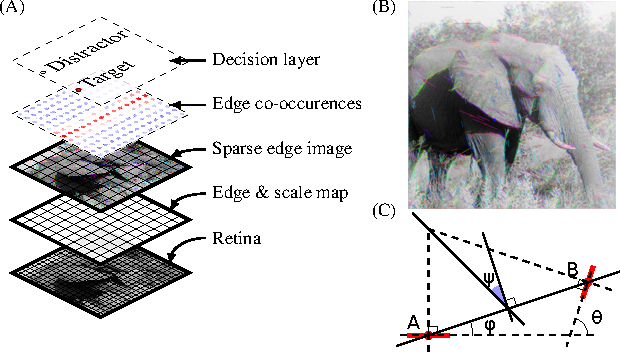
\includegraphics[width=0.8\textwidth]{./classifier.pdf}
	\caption[] {Diagramatic representation of how a classifier is
      trained to distinguish between natural images and inanimate
      objects. A) The different layers used to train the
      classifier. The natural images are first fed through a model
      retina, all the edges are labeled with positions and
      scales. Using a greedy algorithm a set of edges accounting for
      the largest amount of luminance variance within the original
      image are selected. Using this set of edges the edge
      co-occurence statistics were computed and finally the classifier
      was trained based on these statistics. B) The sparse set
      of labelled edges extracted from a single image. C) Diagram
      showing how the angular difference $\theta$ and azimuth angle
      $\phi$ and relative azimuth $\psi$ are computed from two
      edges. Reproduced from \cite{Perrinet2015}.}
	\label{classifier}
\end{figure}

\begin{figure}
	\centering
	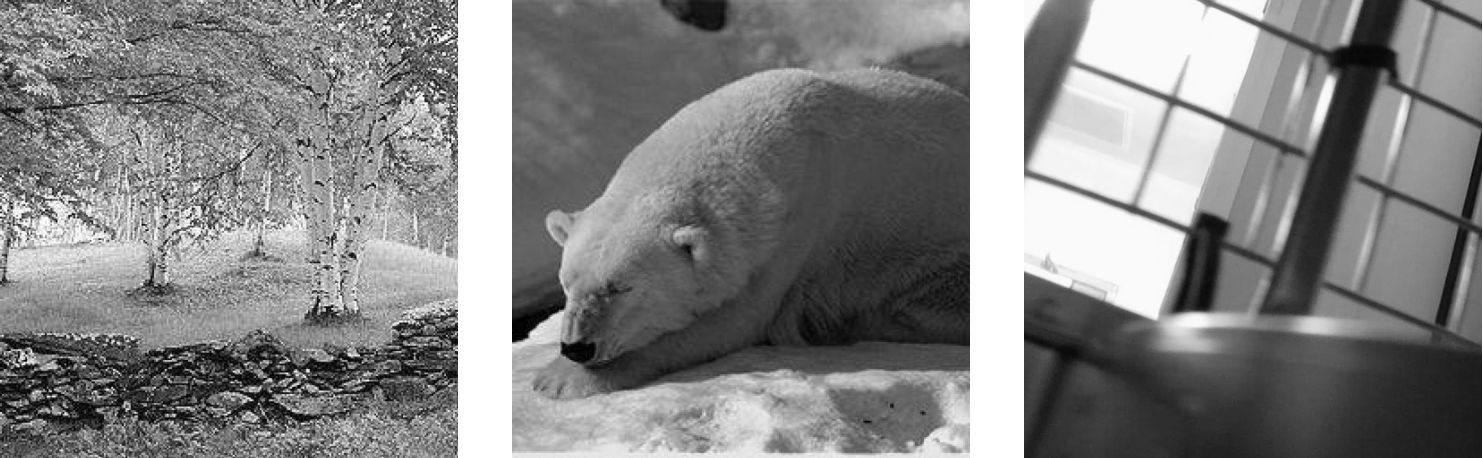
\includegraphics[width=1.0\textwidth]{./image_datasets.pdf}
	\caption[]%
            {The three image datasets used to train the model. From
      left to right 1) Artificial dataset 2) Animal dataset 3) Ferret
      cage dataset.}
    \label{datasets}
\end{figure}

The first step was to train the model on the different image datasets,
which had already been analyzed for their co-occurence statistics (see
figure \ref{classifier}). The datasets fed to the model comprised the
two datasets used as part of the paper and one additional image
dataset recorded in ferret cages, which features great numbers of
extended, high-contrast bars (shown in figure \ref{datasets}).

After training the model independently on each of the datasets the
lateral connection fields were analyzed using a number of novel
analyses. The first analysis that was performed was implemented by
Jean-Luc Stevens and involved aligning the lateral connection field of
each V1Exc neuron along the axis of preferred orientation and
averaging them together. This analysis provides a way to quickly
visually assess whether and how strongly lateral connection fields are
biased along the axis of preferred orientation and is shown in figure
\ref{avg_weights}.

In addition a more detailed analysis, which took into account the
position preference of each pre- and post-synaptic neuron was
implemented. A circular histogram of weight strength was computed by
calculating the azimuth, $\phi$, between the pre- and post-synaptic
neuron for each connection in all the lateral connection fields.

Finally the co-occurence statistics encoded within the lateral
connections were computed. This analysis was largely based around the
\cite{Perrinet2015} code to compute the co-occurence statistics from
sets of sparse labelled edges. As before the azimuth was computed for
all the connections, however additionally the difference in the pre-
and post-synaptic orientation preference $\theta$, angular location of
the second edge relative to the reference edge $\phi$ and the distance
$d$ were calculated. Furthermore we define angle $\psi = \phi
-\theta/2$, which reduces to $\psi = 0$ for co-circular edges. By
binning and weighting each connection weight according to these
properties a co-occurence histogram was computed for various
distances.

It was found that for the distances that are contained within one
lateral field there was very little difference when binning the data
separately, which matches the fact that the classifier employed by
\cite{Perrinet2015} could extract little information from the
distance. In order to reduce the local contribution the central
weights within the same microcolumn were masked out. The resultant
plots are shown in figure \ref{cooccurrence}. Generally a good match is
found between the co-occurence statistics in the dataset and the
statistics encoded in the long-range connections of the model. The
difference is clearest when comparing the laboratory dataset to the
natural dataset, likely because the statistics are so radically
different between these datasets.

\begin{figure}
	\centering
        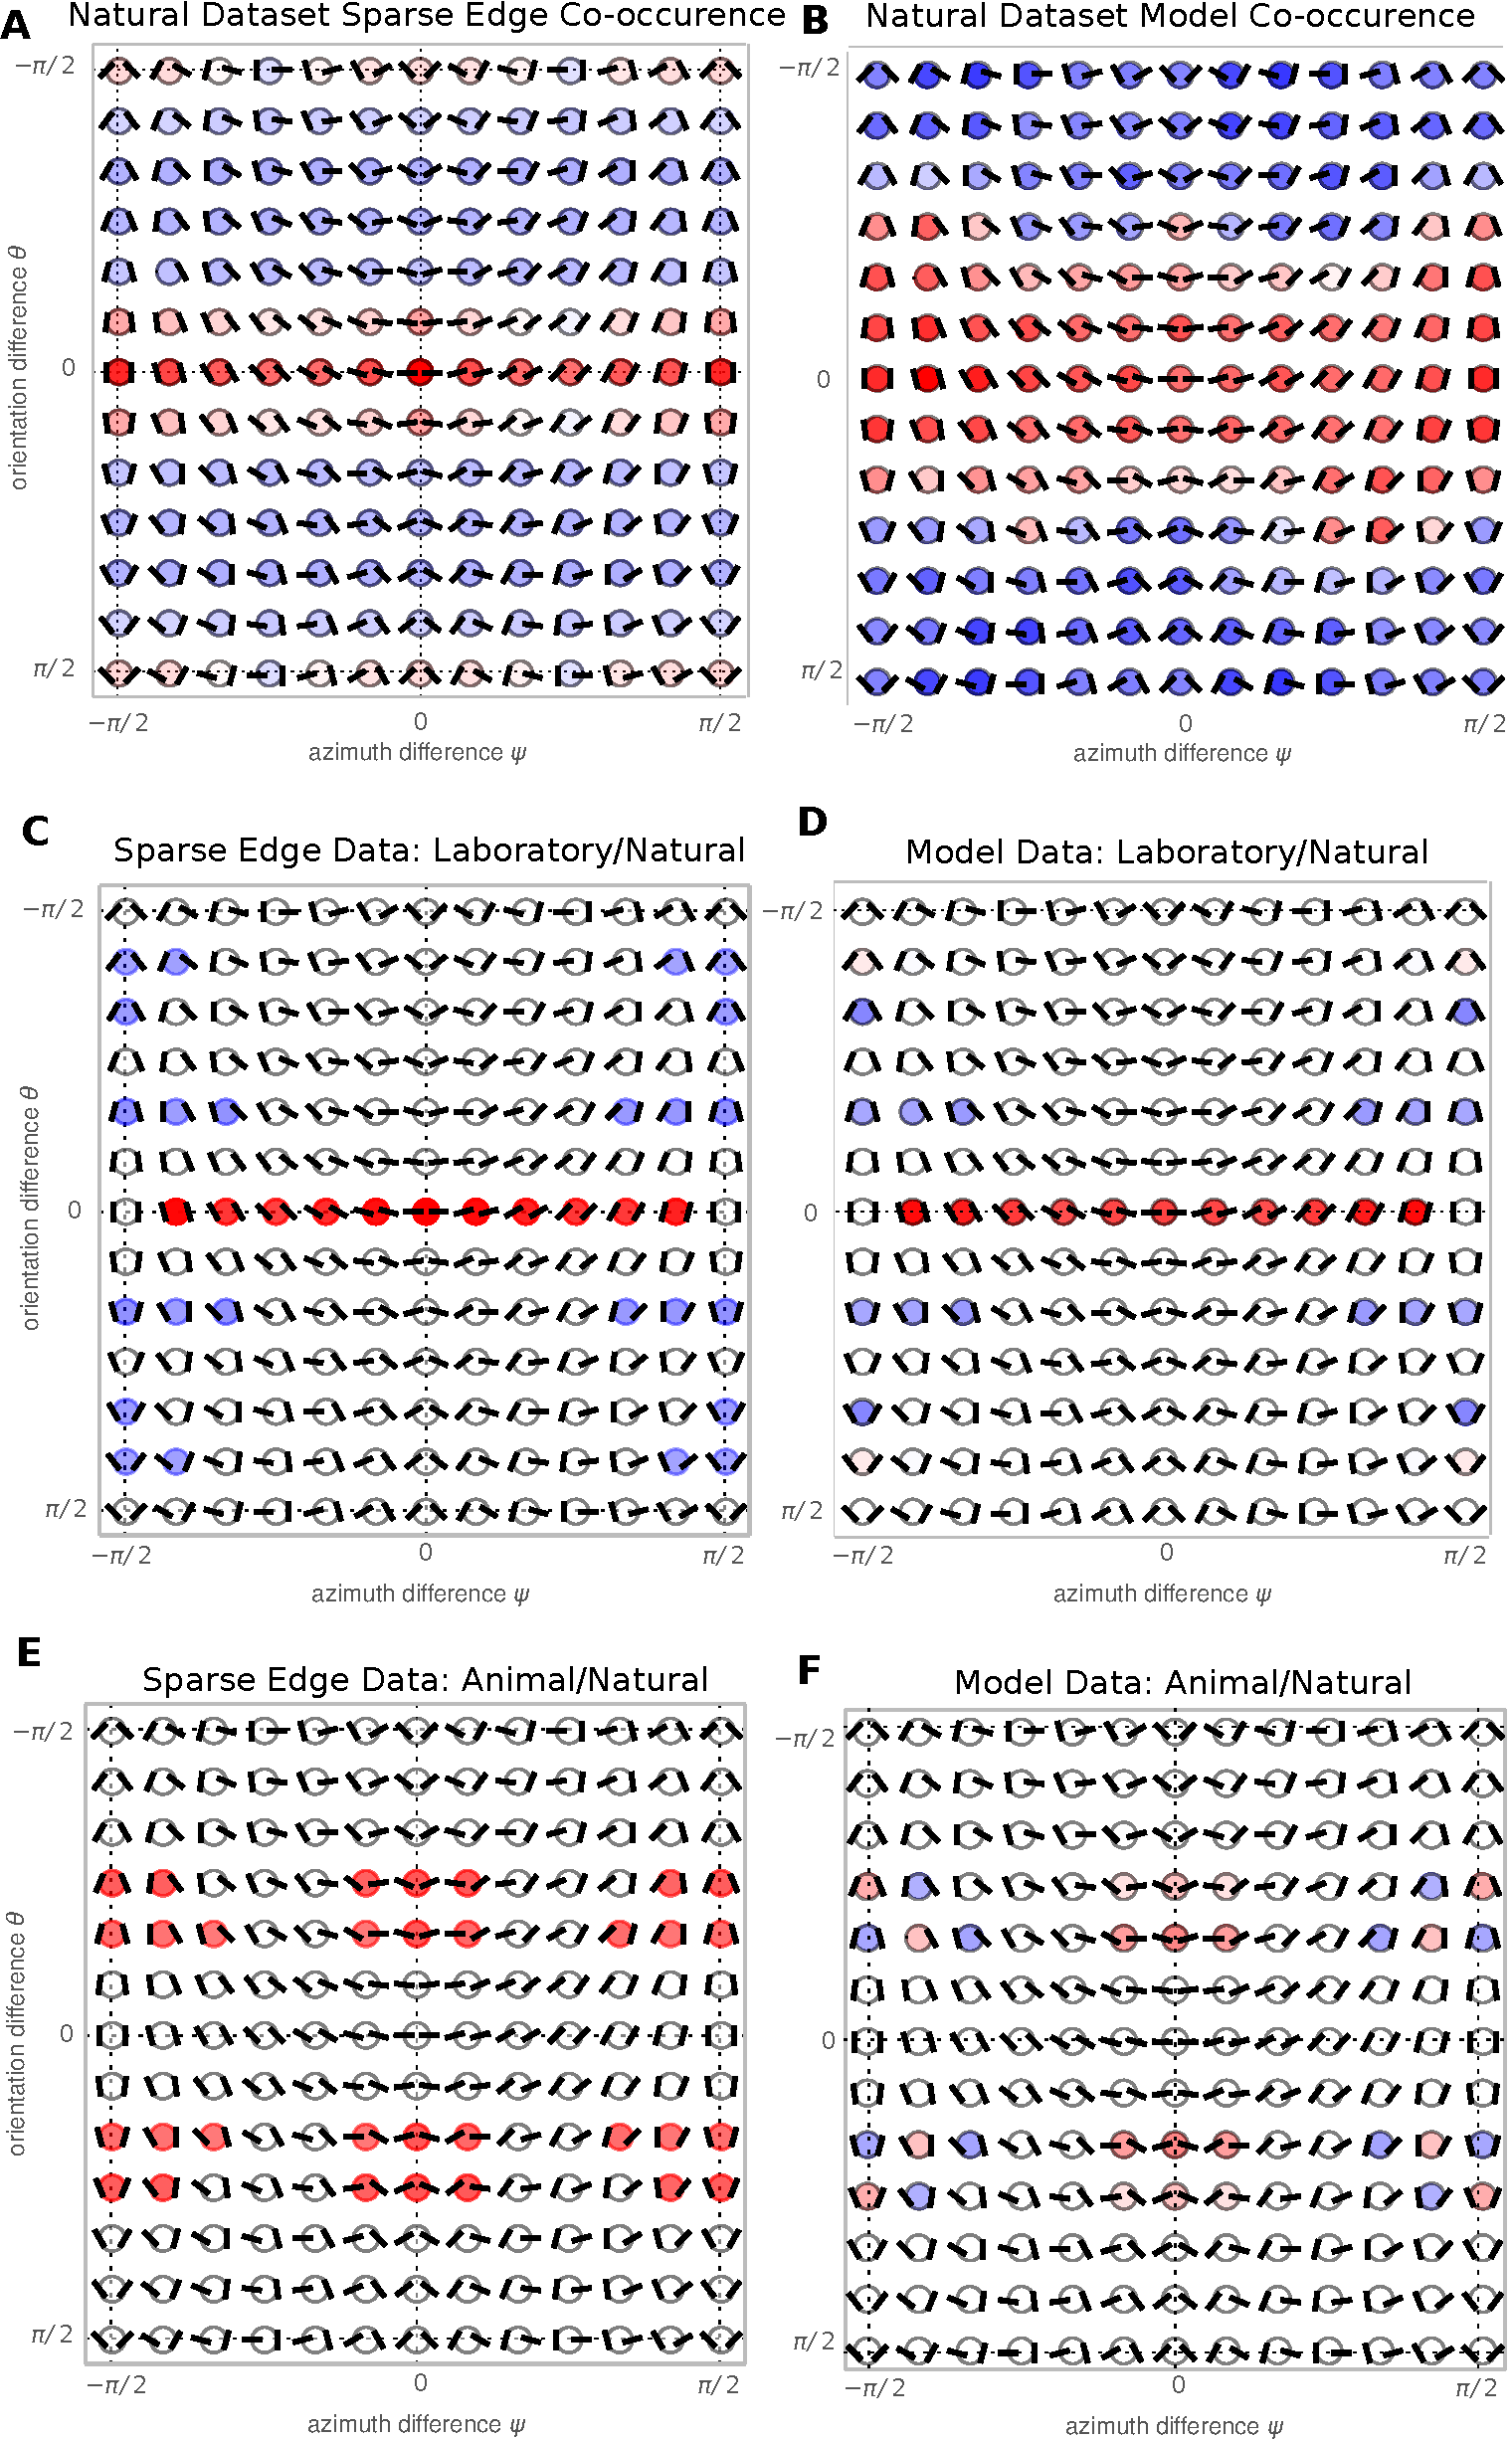
\includegraphics[width=1.0\textwidth]{cooccurrence_plots.pdf}
	\caption{Co-occurence histograms comparing the distribution of
          orientation and relative azimuth of edges extracted from two
          image datasets and the equivalent distribution extracted
          from the lateral connection patterns of the LESPI model,
          highlighting that the model was able to capture the most
          characteristic features of this dataset.}
	\label{cooccurence}
\end{figure}


\begin{itemize}
\item First order orientation distribution
\item Describe Buzas fitting process
\item Describe decoding orientation and azimuth histograms from lateral
  connectivity
\item Describe anisotropy results for different datasets
\item Discuss further work including:
\item Better decoding of position preference
\item Include orientation selectivity in Buzas model
\end{itemize}
